\documentclass[dvipdfmx,10pt]{beamer}


\usepackage{here, amsmath, latexsym, amssymb, bm, ascmac, mathtools, multicol, tcolorbox, subfig, color, tikz, graphics, braket}
\renewcommand{\baselinestretch}{1.2}
\renewcommand{\figurename}{図}
\renewcommand{\tablename}{表}
\renewcommand{\kanjifamilydefault}{\gtdefault}
\usefonttheme{professionalfonts}
\setbeamertemplate{navigation symbols}{}

\usetheme{Boadilla}

\title{ディープラーニングと物理学}
\subtitle{4.2 \ 再帰的ニューラルネットワークと誤差逆伝播法}
\author[須賀]{須賀勇貴}
\institute[茨大]{茨城大学大学院 \ 理工学研究科 \ 量子線科学専攻 \ 2年}
\date{\today}

\begin{document}

\frame{\maketitle}

  \begin{frame}{時系列データについて}
    \begin{block}{系列データ}
      個々の要素が順序付きの集まりとして与えられるデータのこと\\
      (ex) 
      \begin{itemize}
        \item 動画データ $\rightarrow$ 順序付きの自然画像データ
        \item 文章データ $\rightarrow$ 順序付きの文字画像データ
        \item 会話データ $\rightarrow$ 順序付きの音声データ
      \end{itemize}
    \end{block}
    長さが$T$の系列データは以下のように表現できる
      \begin{equation*}
        \begin{pmatrix*}
          x(1) \\ x(2) \\ x(3) \\ \vdots \\ x(T)
        \end{pmatrix*}
        =\ket{x(t)} \ \ (t=1,2,3,\cdots,T)
      \end{equation*}  
  \end{frame}

  \begin{frame}{時系列データについて}
    (ex) "This is an apple ."という文章データを系列データとして扱う場合
    \begin{align*}
      \ket{x(1)} &= \ket{\text{This}}\\
      \ket{x(2)} &= \ket{\text{is}}\\
      \ket{x(3)} &= \ket{\text{an}}\\
      \ket{x(4)} &= \ket{\text{apple}}\\
      \ket{x(5)} &= \ket{\text{.}}
    \end{align*}
    文字データなどは\textbf{1-of-Kベクトル}などにより数値ベクトルとして表現される
    \begin{figure}
      \begin{center}
        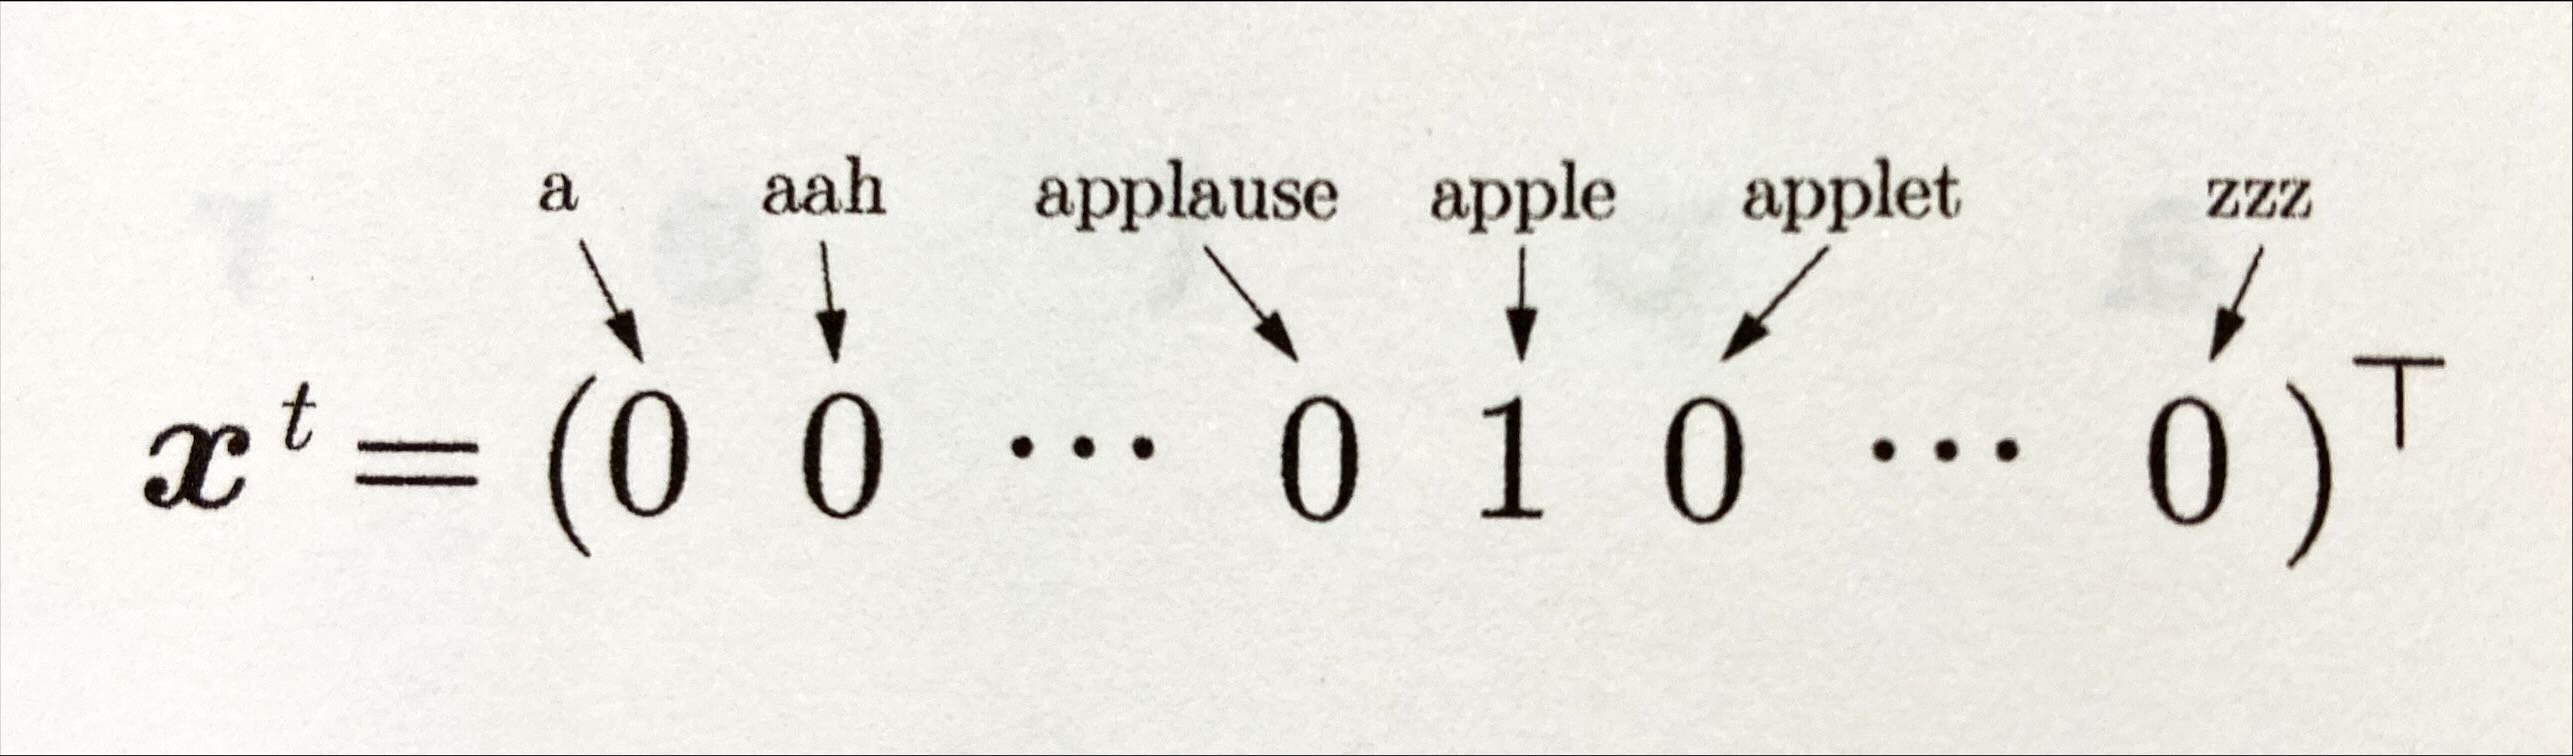
\includegraphics[height=2cm]{apple_vector.jpeg}
      \end{center} 
      \caption{"apple"の1-of-kベクトル表示}  
    \end{figure}
  \end{frame}

  \begin{frame}{再帰的ニューラルネットワーク(RNN)の考え方}
    これまで、扱ってきたデータはデータ間につながりがないものだった
    \begin{center}
      $\Downarrow$
    \end{center}
    系列データをニューラルネットワークで扱えるようにしたい\\
    \begin{center}
      $\Downarrow$
    \end{center}
    データ間のつながりを表現できるようなニューラルネットワークを構築すればよい!
  \end{frame}

  \begin{frame}{再帰的ニューラルネットワーク(RNN)の考え方}
    素朴な考え方\\
    $\Rightarrow$前の時刻の出力を次の時刻の入力に加えるようなニューラルネットワーク
    \begin{figure}
      \begin{center}
        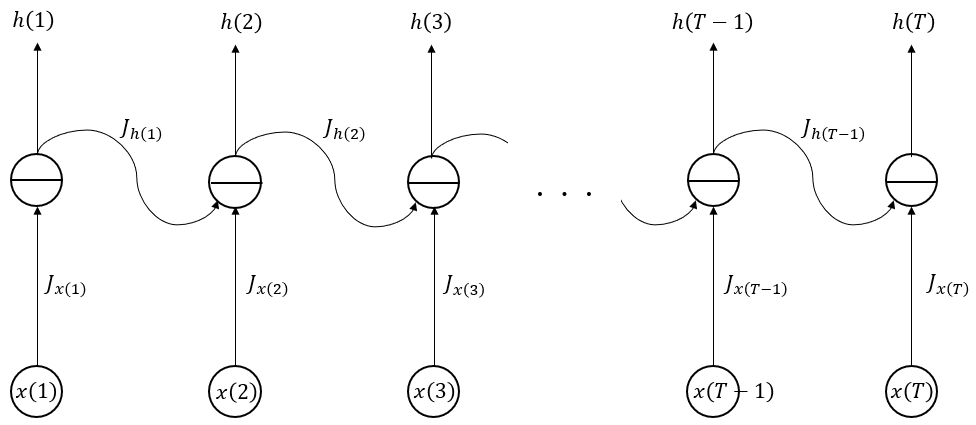
\includegraphics[height=5.2cm]{simple_RNN.png}
      \end{center} 
      \caption{最もシンプルな形のRNN}  
    \end{figure}
  \end{frame}

  \begin{frame}{再帰的ニューラルネットワーク(RNN)の考え方}
    \begin{figure}
      \begin{center}
        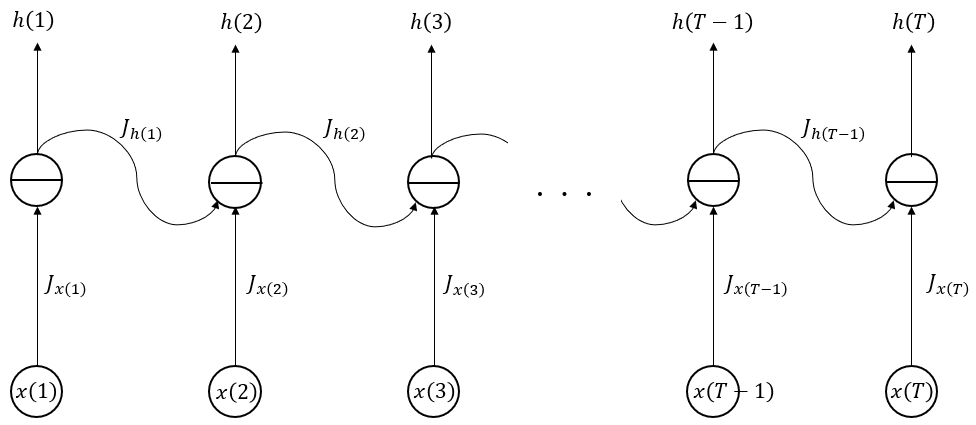
\includegraphics[height=4cm]{simple_RNN.png}
      \end{center} 
    \end{figure}
    以下のようにベクトルや行列で表現しておく
    \begin{align*}
      \ket{x(t)} &= (x(1),x(2),\cdots,x(T))^{\top}\\
      \ket{h(t)} &= (h(1),h(2),\cdots,h(T))^{\top}\\
      \mathbb{J}_x &= \text{diag}(J_{x(1)},J_{x(2)},\cdots,J_{x(T)})\\
      \mathbb{J}_h &= \text{diag}(J_{h(1)},J_{h(2)},\cdots,J_{h(T)})
    \end{align*}
  \end{frame}

  \begin{frame}{再帰的ニューラルネットワーク(RNN)の考え方}
    各時刻での出力は以下のように簡単に求められる
    \begin{align*}
      h(1) &= \sigma_{\bullet}(J_{x(1)}x(1))\\
      h(2) &= \sigma_{\bullet}(J_{x(2)}x(2) + J_{h(1)}h(1))\\
      \vdots\\
      h(t) &= \sigma_{\bullet}(J_{x(t)}(t)x(t) + J_{h(t-1)}h(t-1))
    \end{align*}
    ブラケット表記より,まとめて以下のように書ける
    \begin{align*}
      \ket{h(t)} &= \sigma_{\bullet}(\mathbb{J}_x\ket{x(t)} + \mathbb{J}_h\ket{h(t-1)})\\
      &= \sum_{m}\ket{m}\sigma_{\bullet}\Big(\bra{m}\mathbb{J}_x\ket{x(t)} + \bra{m}\mathbb{J}_h\ket{h(t-1)}\Big)
    \end{align*}
  \end{frame}

  \begin{frame}{再帰的ニューラルネットワーク(RNN)の考え方}
    「ループ」のような構造(=再帰的)を持つニューラルネットワーク\\
    $\Rightarrow$ 再帰的ニューラルネットワーク
    \begin{figure}
      \begin{center}
        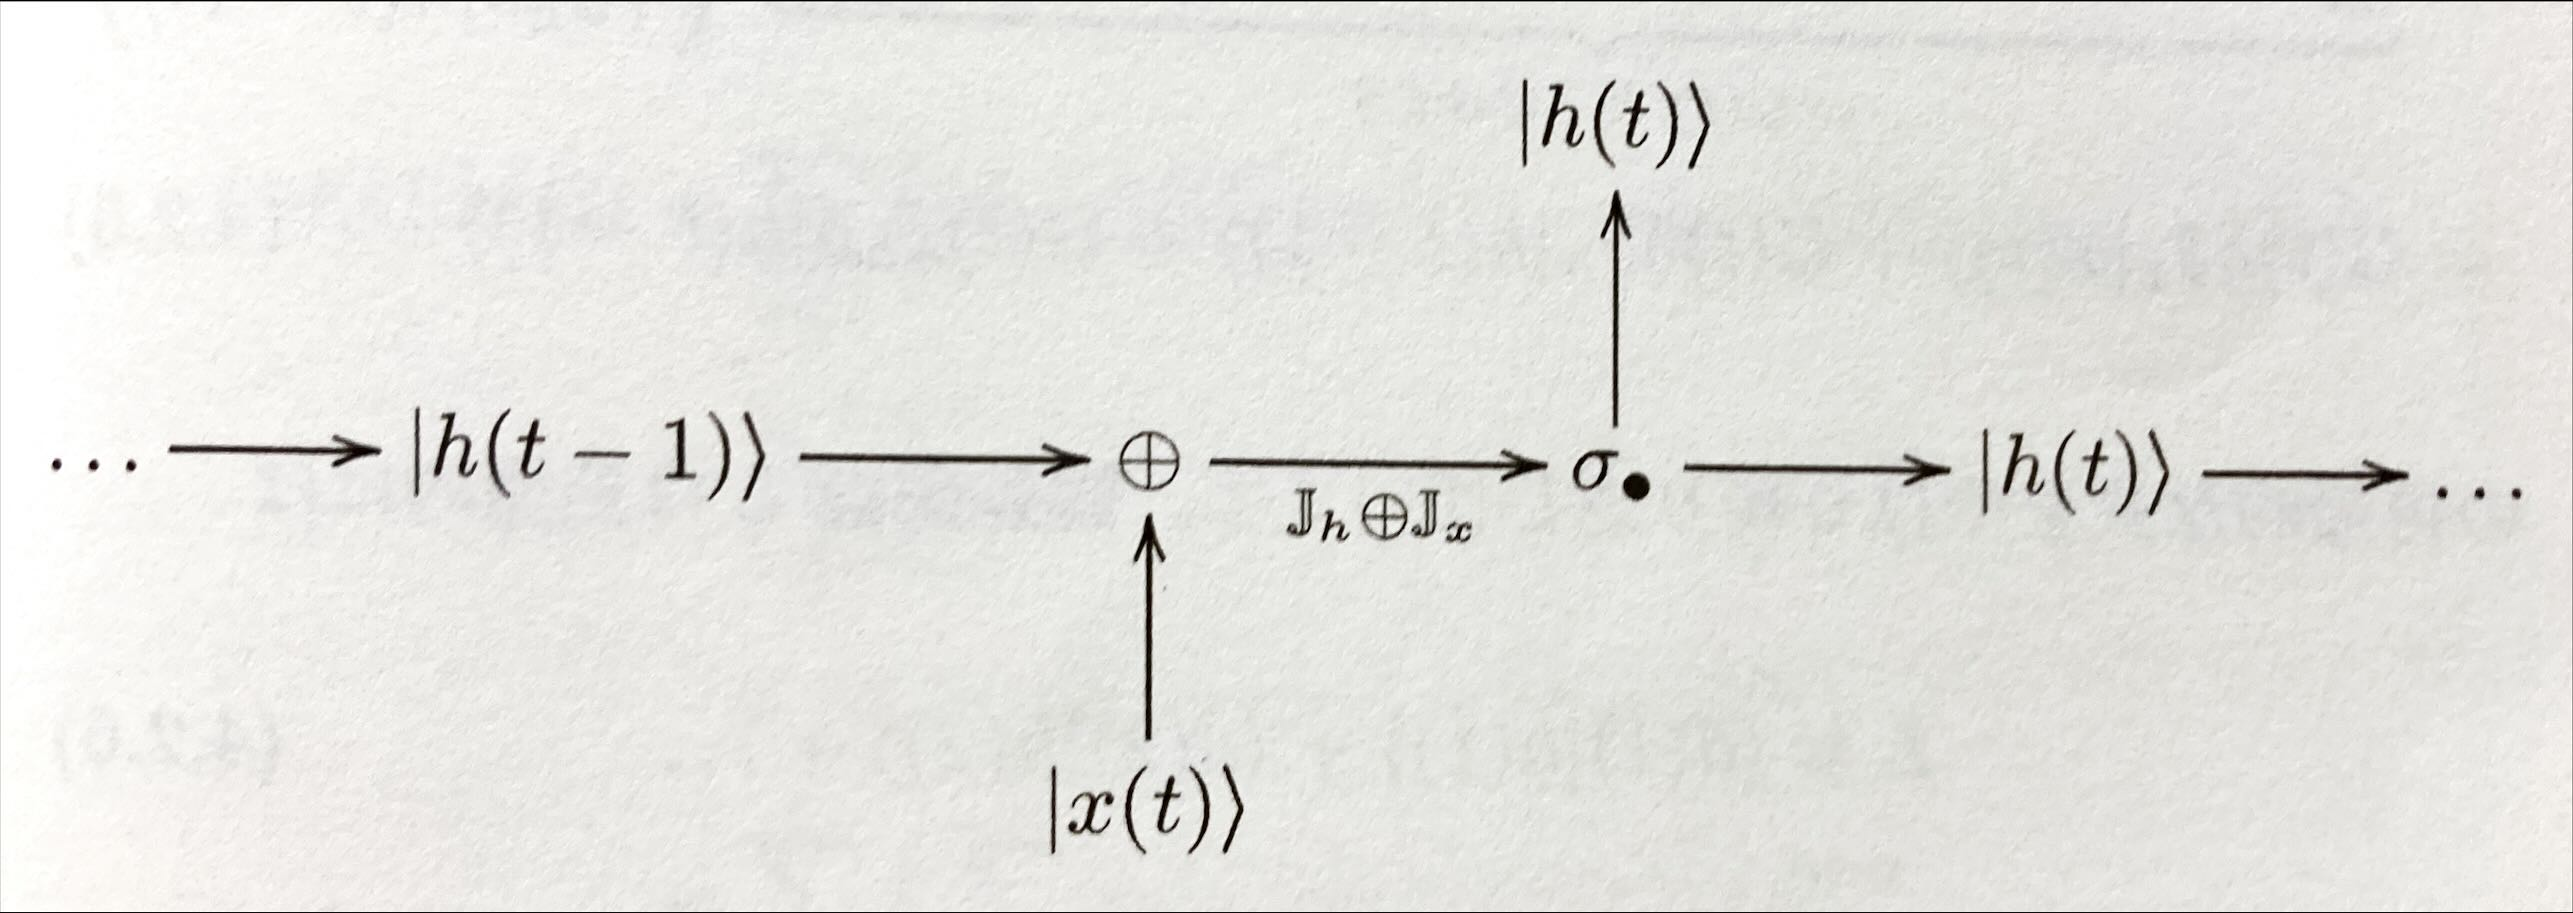
\includegraphics[height=3.5cm]{RNN_diagram.jpeg}
      \end{center}
      \caption{素朴な再帰的ニューラルネットワークの模式図} 
    \end{figure}
    \begin{equation*}
      \ket{h(t)} = \sum_{m}\ket{m}\sigma_{\bullet}\Big(\bra{m}\mathbb{J}_x\ket{x(t)} + \bra{m}\mathbb{J}_h\ket{h(t-1)}\Big)
    \end{equation*}
  \end{frame}

  \begin{frame}{RNNにおける誤差逆伝播}
    誤差関数$L$は典型的に以下のようになっているとする
    \begin{equation*}
      L = \braket{d(1)|h(1)} + \braket{d(2)|h(2)} + \cdots + \braket{d(T)|h(T)}= \sum_{t}\braket{d(t)|h(t)}
    \end{equation*}
    $t$番目の変化量に着目\hyperlink{計算1}{(\text{計算↓})}
    \begin{align*}
      \delta \braket{d(t)|h(t)} 
      &= \bra{d(t)} \delta \ket{h(t)} \ \\
      &= \cdots\\
      &= \bra{\delta_t (t)}\delta \mathbb{J}_x \ket{x(t)} + \bra{\delta_t (t)}\delta \mathbb{J}_h \ket{h(t-1)}\\
      &+ \bra{\delta_t (t-1)}\delta \mathbb{J}_x \ket{x(t-1)} + \bra{\delta_t (t-1)}\delta \mathbb{J}_h \ket{h(t-2)}\\
      &+ \cdots\\
      &+ \bra{\delta_t (1)}\delta \mathbb{J}_x \ket{x(1)} + \bra{\delta_t (1)}\delta \mathbb{J}_h \ket{h(0)}\\
      &= \sum_{\tau \leq t} \Big(\bra{\delta_t (\tau)}\delta \mathbb{J}_x \ket{x(\tau)} + \bra{\delta_t (\tau)}\delta \mathbb{J}_h \ket{h(\tau-1)} \Big)
    \end{align*}
    
  \end{frame}

  \begin{frame}{RNNにおける誤差逆伝播}
    ここで,
    \begin{equation*}
      \delta \mathbb{J} = \sum_{m,n} \ket{m}\bra{n}\delta J~{mn}
    \end{equation*}
    とすると
    \begin{align*}
      &\delta \braket{d(t)|h(t)} \\
      &= \sum_{\tau \leq t} \Big(\bra{\delta_t (\tau)}\delta \mathbb{J}_x \ket{x(\tau)} + \bra{\delta_t (\tau)}\delta \mathbb{J}_h \ket{h(\tau-1)} \Big)\\
      &= \sum_{\tau \leq t} \sum_{m,n} \Big( \braket{\delta_t (\tau)|m} \braket{n|x(\tau)}\delta J_x^{mn} + \braket{\delta_t (\tau)|m} \braket{n|h(\tau-1)}\delta J_h^{mn} \Big)\\
      &= \sum_{m,n} \Big( \sum_{\tau \leq t} \braket{\delta_t (\tau)|m} \braket{n|x(\tau)}\delta J_x^{mn} + \sum_{\tau \leq t} \braket{\delta_t (\tau)|m} \braket{n|h(\tau-1)}\delta J_h^{mn} \Big)
    \end{align*}
  \end{frame}

  \begin{frame}{RNNにおける誤差逆伝播}
    以上の結果から誤差関数$L$の変化量は
    \begin{align*}
      \delta L 
      &= \sum_{t}\delta\braket{d(t)|h(t)}\\
      &= \sum_{m,n} \Big( \sum_{t}\sum_{\tau \leq t} \braket{\delta_t (\tau)|m} \braket{n|x(\tau)}\delta J_x^{mn}\\
      &\hspace{0.8cm}+ \sum_{t}\sum_{\tau \leq t} \braket{\delta_t (\tau)|m} \braket{n|h(\tau-1)}\delta J_h^{mn} \Big)
    \end{align*}
    と表すことができる.この結果より,パラメータ$J_x^{mn}$と$J_h^{mn}$はそれぞれ
    \begin{align*}
      \delta J_x^{mn} &= -\epsilon \sum_{t}\sum_{\tau \leq t} \braket{\delta_t (\tau)|m} \braket{n|x(\tau)}\\
      \delta J_h^{mn} &= -\epsilon \sum_{t}\sum_{\tau \leq t} \braket{\delta_t (\tau)|m} \braket{n|h(\tau-1)}
    \end{align*}
    という更新ルールにすれば,誤差関数の値が小さくなるようになる.
  \end{frame}

  \begin{frame}{RNNにおける誤差逆伝播}
    (check)
    \begin{align*}
      &\delta L = -\epsilon \sum_{n,m} \\
      &\times \underbrace{\Big[ \Big( \sum_t \sum_{\tau \leq t} \braket{\delta_t(\tau)|m}\braket{n|x(\tau)} \Big)^2 + \Big( \sum_t \sum_{\tau \leq t} \braket{\delta_t(\tau)|m}\braket{n|h(\tau-1)} \Big)^2 \Big]}_{>0}\\
      &<0
    \end{align*}
    今回の場合,逆伝播の式は以下
    \begin{align*}
      \bra{\delta_t (\tau-1)} &= \bra{\delta_t (\tau)}\mathbb{J}_h \mathbb{G}(\tau-1)\\
      \bra{\delta_t (t)} &= \bra{d(t)}\mathbb{G}(t)
    \end{align*}
  \end{frame}

  \begin{frame}{勾配爆発/勾配消失}
    ここで考えた再帰的ニューラルネットワークでは勾配爆発か勾配消失のどちらかが起こってしまい,うまく学習することができないという問題がある.\\
    \vspace{0.3cm}
    逆伝播のより
    \begin{align*}
      \bra{\delta_t (1)}
      &= \bra{\delta_t (2)}\mathbb{J}_h \mathbb{G}(1) = \bra{\delta_t (3)} \mathbb{J}_h \mathbb{G}(2) \mathbb{J}_h \mathbb{G}(1)\\
      &= \cdots\\
      &= \bra{d(T)}\mathbb{G}(T) \mathbb{J}_h \mathbb{G}(T-1) \cdots \mathbb{J}_h \mathbb{G}(2) \mathbb{J}_h \mathbb{G}(1)
    \end{align*}
    $\Rightarrow$ $\mathbb{J}_h$が右から$T-1$回右から作用することになる\\
    \vspace{0.3cm}
    文章データを扱うのであれば$T$は文章の単語数などに対応する\\
    $\rightarrow$1000単語ある文章を学習するとなるとがほぼ1000回かかることになる
  \end{frame}

  \begin{frame}{勾配爆発/勾配消失}
    \begin{align*}
      |\mathbb{J}_h| &> 1 : \bra{\delta_t(1)}\text{が巨大すぎる}\\
      |\mathbb{J}_h| &< 1 : \bra{\delta_t(1)}\text{が小さすぎる}
    \end{align*}
  \end{frame}


  \begin{frame}[label=計算1]{$\delta\ket{h(t)}$の計算}
    パラメータに依存するのは$\mathbb{J}_{x,h}$と$\ket{h(t-1)}$なので
    \begin{align*}
      \delta \ket{h(t)} &= \underbrace{\sum_{m}\ket{m}\sigma'_{\bullet}\Big(\bra{m}\mathbb{J}_{x}\ket{x(t)} + \bra{m}\mathbb{J}_{h}\ket{h(t-1)}\Big)\bra{m}}_{\eqcolon \mathbb{G}(t)}\\
      &\times \delta \Big(\mathbb{J}_x\ket{x(t)} + \mathbb{J}_{h}\ket{h(t-1)}\Big)\\
      &= \mathbb{G}(t)\Big( \delta \mathbb{J}_x \ket{x(t)} + \delta \mathbb{J}_{h}\ket{h(t-1)} + \mathbb{J}_{h}\delta\ket{h(t-1)} \Big)\\
      &= \mathbb{G}(t)\delta \mathbb{J}_x \ket{x(t)} + \mathbb{G}(t)\delta\mathbb{J}_h\ket{h(t-1)} + \mathbb{G}(t)\mathbb{J}_h \delta \ket{h(t-1)}
    \end{align*}
  \end{frame}


\end{document}